\chapter{Event-Driven Architecture}
\authors{Delvin, Gabrielle Sheila Sylvagno, Danica Recca Danendra}


\section{Event-Driven Architecture}
\subsection{Event-Driven Architecture}
\begin{figure}[h]
	\centering
	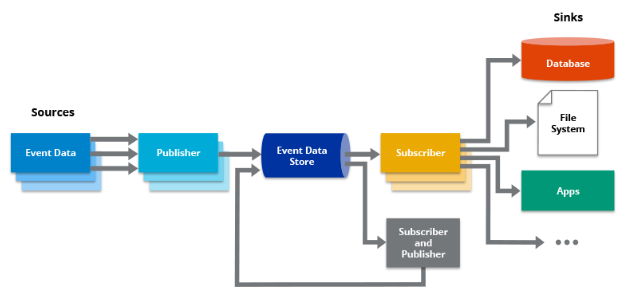
\includegraphics[width=\textwidth]{diagram-EDA}
	\caption{Skema Diagram EDA}
	\label{fig:diagram-EDA}
\end{figure}
\textit{Event-driven architecture} (EDA) atau arsitektur berbasis peristiwa adalah paradigma desain perangkat lunak yang memanfaatkan peristiwa \textit{(event)} sebagai dasar interaksi dan integrasi antara komponen-komponen perangkat lunak.EDA berfokus pada peristiwa yang terjadi pada waktu tertentu, seperti permintaan pengguna atau respons sistem terhadap permintaan tersebut. Komponen-komponen perangkat lunak dalam arsitektur ini saling berkomunikasi melalui peristiwa-peristiwa yang terjadi, sehingga memungkinkan sistem untuk beroperasi secara asinkron.EDA sering digunakan dalam pengembangan aplikasi skala besar dan sistem berbasis layanan \textit{ (service-oriented architecture/SOA)} untuk memastikan penggunaan sumber daya yang efektif dan efisien. Arsitektur ini juga dapat membantu meminimalkan waktu respon dan meningkatkan skalabilitas sistem.Berikut ini diagram EDA yang ditampilkan pada \ref{fig:diagram-EDA}


\section{Kelebihan dan Kekurangan}
\subsection{Kelebihan}
Berikut ini adalah kelebihan dari EDA:
\begin{itemize}
\item Asinkron: EDA memungkinkan komponen sistem beroperasi secara asinkron, yaitu mereka dapat beroperasi secara independen tanpa harus menunggu komponen lainnya untuk menyelesaikan tugasnya.	
\item Pemicu: EDA didasarkan pada penggunaan peristiwa sebagai pemicu untuk memicu tindakan atau respons. Ketika peristiwa terjadi, EDA akan memicu tindakan yang sesuai dengan peristiwa tersebut.	
\item Publikasi dan Langganan: EDA menggunakan model publikasi-langganan \textit{(publish-subscribe)} dimana sebuah komponen menghasilkan peristiwa \textit{(publisher)} dan komponen lainnya yang tertarik \textit{(subscriber)} dapat menerima dan menangani peristiwa tersebut.	
\item Terdistribusi: EDA memungkinkan komponen sistem tersebar di berbagai mesin atau jaringan, sehingga memudahkan pengembangan sistem yang \textit{scalable} dan tahan bencana.	

\item Flesksibel dan modular: EDA
memisahkan komponen-komponen sistem sehingga mereka dapat beroperasi secara independen dan dapat digunakan kembali dalam berbagai aplikasi atau sistem yang berbeda.	
\item Responsif: EDA memungkinkan sistem merespons permintaan dengan cepat, karena komponen sistem dapat beroperasi secara independen dan merespons peristiwa secara asinkron.	
\item Berorientasi pada pesan: EDA menggunakan pesan sebagai sarana untuk berkomunikasi antar komponen sistem. Pesan dapat mengandung data atau informasi yang diperlukan oleh komponen lain dalam sistem.	
\item Skalabel: EDA dapat diimplementasikan pada sistem yang memiliki tingkat skala dan kompleksitas yang berbeda-beda, mulai dari sistem skala kecil hingga sistem skala besar dan terdistribusi.
\end{itemize}

\subsection{Kekurangan}
Berikut ini adalah kekurangan dari EDA:
\begin{itemize}
\item Kompleksitas: EDA bisa menjadi sangat kompleks karena banyaknya komponen dan interaksi antar komponen dalam sistem. Hal ini dapat membuat pengembangan dan pemeliharaan sistem menjadi lebih sulit.	
\item Kesulitan dalam pemantauan dan manajemen: Dalam EDA, setiap peristiwa dapat dicatat dan dilacak, namun hal ini bisa menyebabkan sulitnya pemantauan dan manajemen sistem jika terdapat banyak peristiwa yang terjadi pada waktu yang sama.	
\item Kemungkinan kesalahan: Karena EDA melibatkan banyak komponen yang berinteraksi satu sama lain, maka kemungkinan terjadinya kesalahan atau bug dalam sistem juga semakin besar. Hal ini dapat menyebabkan kerusakan sistem atau bahkan kegagalan total dalam sistem.
/item Tidak cocok untuk sistem yang simpel: EDA biasanya digunakan pada sistem yang kompleks dan memerlukan integrasi dengan berbagai sistem atau aplikasi lainnya. Sehingga EDA mungkin tidak cocok untuk sistem yang simpel atau terbatas dalam kompleksitasnya.
\end{itemize}

\section{Contoh Penerapan}
	\subsection{Perbankan}
 Sistem perbankan: EDA dapat digunakan untuk membangun sistem perbankan yang responsif dan skalabel. Contohnya adalah ketika seorang pelanggan melakukan transfer uang, hal ini memicu peristiwa (event) yang kemudian membuat sistem mengirimkan notifikasi kepada penerima transfer bahwa uang telah diterima.
\subsection{E-commerce}
 Aplikasi e-commerce: EDA dapat digunakan dalam aplikasi e-commerce untuk mempercepat proses pembelian. Ketika seorang pelanggan menyelesaikan pembelian, peristiwa ini dapat memicu sistem untuk mengirim notifikasi ke bagian pengiriman dan bagian keuangan untuk memproses pesanan.
\subsection{Internet of Thing (IoT)}
 Internet of Things (IoT): EDA juga dapat digunakan dalam sistem IoT, di mana banyak sensor dan perangkat harus berinteraksi dengan sistem pusat. Contohnya adalah ketika suhu di suatu ruangan melebihi batas normal, peristiwa ini dapat memicu sistem untuk mengirim notifikasi ke teknisi untuk memperbaiki perangkat pendingin ruangan.
\subsection{Manajemen Rantai Pasokan}
 Sistem manajemen rantai pasokan: EDA dapat digunakan dalam sistem manajemen rantai pasokan untuk memantau pergerakan barang dari satu titik ke titik lainnya. Ketika sebuah produk telah dikirim, peristiwa ini dapat memicu sistem untuk mengirim notifikasi ke penerima produk tentang waktu pengiriman yang dijadwalkan.
 \subsection{Manajemen Proyek}
 Sistem manajemen proyek: EDA dapat digunakan dalam sistem manajemen proyek untuk memantau perkembangan proyek dan memperingatkan manajer proyek ketika terjadi masalah atau penundaan. Contohnya, ketika seorang anggota tim menyelesaikan tugas mereka, peristiwa ini dapat memicu sistem untuk memperbarui proyek secara otomatis dan memberikan notifikasi kepada manajer proyek.




